% Se incluye el preambulo del trabajo
% Se configura el tipo de documento
\documentclass[a4paper]{article}

% Paquetes utilizados
\usepackage[utf8]{inputenc}
\usepackage[spanish, es-tabla]{babel}
\usepackage{float}
\usepackage{graphicx}
\usepackage{subcaption}

% Paquetes de matematica
\usepackage{amsmath}
\usepackage{steinmetz}

% Paquetes para excel
\usepackage{csvsimple}

% Configuracion del informe
\setlength{\parindent}{0pt}
\setcounter{secnumdepth}{0}

\usepackage[a4paper, 
    includehead, 
    footskip=7mm, 
    headsep=6mm, 
    headheight=4.8mm,
    top=25mm, bottom=25mm, left=25mm, right=25mm]{geometry}

%THIS IS FOR SETTING LOCATION OF FLOATS
\usepackage{float}
%ENDS SETTING LOCATION OF FLOATS

%THE FOLLOWING ARE CONFIGURATIONS FOR TODONOTES
\usepackage{todonotes,varwidth}
\makeatletter
\tikzstyle{diaanotestyle} = [
    draw=\@todonotes@currentbordercolor,
    fill=\@todonotes@currentbackgroundcolor,
    line width=0.5pt,
    inner sep = 0.8 ex,
    rounded corners=4pt,align=left,
   ]

\renewcommand{\@todonotes@drawInlineNote}{%
        {\begin{tikzpicture}[remember picture,baseline={(0,0)}]%
            \draw node[diaanotestyle,font=\@todonotes@sizecommand,anchor=base west]{%
               \begin{varwidth}[t]{10cm}
                \if@todonotes@authorgiven%
                    {\@todonotes@sizecommand \@todonotes@author:\,\@todonotes@text}%
                \else%
                    {\@todonotes@sizecommand \@todonotes@text}%
                \fi
                \end{varwidth}};%
            \end{tikzpicture}}%
       }%
\makeatother
%HERE ENDS THE CONFIGURATIONS FOR TODONOTES

%THE FOLLOWING ARE CONFIGURATIONS FOR LISTINGS (to insert code)
\usepackage{listings}

\definecolor{dkgreen}{rgb}{0,0.6,0}
\definecolor{gray}{rgb}{0.5,0.5,0.5}
\definecolor{mauve}{rgb}{0.58,0,0.82}

\lstset{frame=tb,
  language=Bash,
  aboveskip=3mm,
  belowskip=3mm,
  showstringspaces=false,
  columns=flexible,
  basicstyle={\small\ttfamily},
  numbers=none,
  numberstyle=\tiny\color{gray},
  keywordstyle=\color{blue},
  commentstyle=\color{dkgreen},
  stringstyle=\color{mauve},
  breaklines=true,
  breakatwhitespace=true,
  tabsize=3
}
%HERE ENDS THE CONFIGURATIONS FOR LISTINGS


\usepackage{hyperref}
\hypersetup{
    colorlinks=true,
    linkcolor=blue,
    filecolor=magenta,      
    urlcolor=blue,
    citecolor=blue,    
}

%MAPAS DE KARNAUGH
\usepackage{tikz}
\usetikzlibrary{matrix,calc}

%isolated term
%#1 - Optional. Space between node and grouping line. Default=0
%#2 - node
%#3 - filling color
\newcommand{\implicantsol}[3][0]{
    \draw[rounded corners=3pt, fill=#3, opacity=0.3] ($(#2.north west)+(135:#1)$) rectangle ($(#2.south east)+(-45:#1)$);
    }


%internal group
%#1 - Optional. Space between node and grouping line. Default=0
%#2 - top left node
%#3 - bottom right node
%#4 - filling color
\newcommand{\implicant}[4][0]{
    \draw[rounded corners=3pt, fill=#4, opacity=0.3] ($(#2.north west)+(135:#1)$) rectangle ($(#3.south east)+(-45:#1)$);
    }

%group lateral borders
%#1 - Optional. Space between node and grouping line. Default=0
%#2 - top left node
%#3 - bottom right node
%#4 - filling color
\newcommand{\implicantcostats}[4][0]{
    \draw[rounded corners=3pt, fill=#4, opacity=0.3] ($(rf.east |- #2.north)+(90:#1)$)-| ($(#2.east)+(0:#1)$) |- ($(rf.east |- #3.south)+(-90:#1)$);
    \draw[rounded corners=3pt, fill=#4, opacity=0.3] ($(cf.west |- #2.north)+(90:#1)$) -| ($(#3.west)+(180:#1)$) |- ($(cf.west |- #3.south)+(-90:#1)$);
}

%group top-bottom borders
%#1 - Optional. Space between node and grouping line. Default=0
%#2 - top left node
%#3 - bottom right node
%#4 - filling color
\newcommand{\implicantdaltbaix}[4][0]{
    \draw[rounded corners=3pt, fill=#4, opacity=0.3] ($(cf.south -| #2.west)+(180:#1)$) |- ($(#2.south)+(-90:#1)$) -| ($(cf.south -| #3.east)+(0:#1)$);
    \draw[rounded corners=3pt, fill=#4, opacity=0.3] ($(rf.north -| #2.west)+(180:#1)$) |- ($(#3.north)+(90:#1)$) -| ($(rf.north -| #3.east)+(0:#1)$);
}

%group corners
%#1 - Optional. Space between node and grouping line. Default=0
%#2 - filling color
\newcommand{\implicantcantons}[2][0]{
    \draw[rounded corners=3pt, opacity=.3] ($(rf.east |- 0.south)+(-90:#1)$) -| ($(0.east |- cf.south)+(0:#1)$);
    \draw[rounded corners=3pt, opacity=.3] ($(rf.east |- 8.north)+(90:#1)$) -| ($(8.east |- rf.north)+(0:#1)$);
    \draw[rounded corners=3pt, opacity=.3] ($(cf.west |- 2.south)+(-90:#1)$) -| ($(2.west |- cf.south)+(180:#1)$);
    \draw[rounded corners=3pt, opacity=.3] ($(cf.west |- 10.north)+(90:#1)$) -| ($(10.west |- rf.north)+(180:#1)$);
    \fill[rounded corners=3pt, fill=#2, opacity=.3] ($(rf.east |- 0.south)+(-90:#1)$) -|  ($(0.east |- cf.south)+(0:#1)$) [sharp corners] ($(rf.east |- 0.south)+(-90:#1)$) |-  ($(0.east |- cf.south)+(0:#1)$) ;
    \fill[rounded corners=3pt, fill=#2, opacity=.3] ($(rf.east |- 8.north)+(90:#1)$) -| ($(8.east |- rf.north)+(0:#1)$) [sharp corners] ($(rf.east |- 8.north)+(90:#1)$) |- ($(8.east |- rf.north)+(0:#1)$) ;
    \fill[rounded corners=3pt, fill=#2, opacity=.3] ($(cf.west |- 2.south)+(-90:#1)$) -| ($(2.west |- cf.south)+(180:#1)$) [sharp corners]($(cf.west |- 2.south)+(-90:#1)$) |- ($(2.west |- cf.south)+(180:#1)$) ;
    \fill[rounded corners=3pt, fill=#2, opacity=.3] ($(cf.west |- 10.north)+(90:#1)$) -| ($(10.west |- rf.north)+(180:#1)$) [sharp corners] ($(cf.west |- 10.north)+(90:#1)$) |- ($(10.west |- rf.north)+(180:#1)$) ;
}

%Empty Karnaugh map 4x4
\newenvironment{Karnaugh}%
{
\begin{tikzpicture}[baseline=(current bounding box.north),scale=0.8]
\draw (0,0) grid (4,4);
\draw (0,4) -- node [pos=0.7,above right,anchor=south west] {AB} node [pos=0.7,below left,anchor=north east] {CD} ++(135:1);
%
\matrix (mapa) [matrix of nodes,
        column sep={0.8cm,between origins},
        row sep={0.8cm,between origins},
        every node/.style={minimum size=0.3mm},
        anchor=8.center,
        ampersand replacement=\&] at (0.5,0.5)
{
                       \& |(c00)| 00         \& |(c01)| 01         \& |(c11)| 11         \& |(c10)| 10         \& |(cf)| \phantom{00} \\
|(r00)| 00             \& |(0)|  \phantom{0} \& |(1)|  \phantom{0} \& |(3)|  \phantom{0} \& |(2)|  \phantom{0} \&                     \\
|(r01)| 01             \& |(4)|  \phantom{0} \& |(5)|  \phantom{0} \& |(7)|  \phantom{0} \& |(6)|  \phantom{0} \&                     \\
|(r11)| 11             \& |(12)| \phantom{0} \& |(13)| \phantom{0} \& |(15)| \phantom{0} \& |(14)| \phantom{0} \&                     \\
|(r10)| 10             \& |(8)|  \phantom{0} \& |(9)|  \phantom{0} \& |(11)| \phantom{0} \& |(10)| \phantom{0} \&                     \\
|(rf) | \phantom{00}   \&                    \&                    \&                    \&                    \&                     \\
};
}%
{
\end{tikzpicture}
}

%Empty Karnaugh map 2x4
\newenvironment{Karnaughvuit}%
{
\begin{tikzpicture}[baseline=(current bounding box.north),scale=0.8]
\draw (0,0) grid (4,2);
\draw (0,2) -- node [pos=0.7,above right,anchor=south west] {$y_2 y_1$} node [pos=0.7,below left,anchor=north east] {$w$} ++(135:1);
%
\matrix (mapa) [matrix of nodes,
        column sep={0.8cm,between origins},
        row sep={0.8cm,between origins},
        every node/.style={minimum size=0.3mm},
        anchor=4.center,
        ampersand replacement=\&] at (0.5,0.5)
{
                      \& |(c00)| 00         \& |(c01)| 01         \& |(c11)| 11         \& |(c10)| 10         \& |(cf)| \phantom{00} \\
|(r00)| 0             \& |(0)|  \phantom{0} \& |(1)|  \phantom{0} \& |(3)|  \phantom{0} \& |(2)|  \phantom{0} \&                     \\
|(r01)| 1             \& |(4)|  \phantom{0} \& |(5)|  \phantom{0} \& |(7)|  \phantom{0} \& |(6)|  \phantom{0} \&                     \\
|(rf) | \phantom{00}  \&                    \&                    \&                    \&                    \&                     \\
};
}%
{
\end{tikzpicture}
}

%Empty Karnaugh map 2x2
\newenvironment{Karnaughquatre}%
{
\begin{tikzpicture}[baseline=(current bounding box.north),scale=0.8]
\draw (0,0) grid (2,2);
\draw (0,2) -- node [pos=0.7,above right,anchor=south west] {b} node [pos=0.7,below left,anchor=north east] {a} ++(135:1);
%
\matrix (mapa) [matrix of nodes,
        column sep={0.8cm,between origins},
        row sep={0.8cm,between origins},
        every node/.style={minimum size=0.3mm},
        anchor=2.center,
        ampersand replacement=\&] at (0.5,0.5)
{
          \& |(c00)| 0          \& |(c01)| 1  \\
|(r00)| 0 \& |(0)|  \phantom{0} \& |(1)|  \phantom{0} \\
|(r01)| 1 \& |(2)|  \phantom{0} \& |(3)|  \phantom{0} \\
};
}%
{
\end{tikzpicture}
}

%Defines 8 or 16 values (0,1,X)
\newcommand{\contingut}[1]{%
\foreach \x [count=\xi from 0]  in {#1}
     \path (\xi) node {\x};
}

%Places 1 in listed positions
\newcommand{\minterms}[1]{%
    \foreach \x in {#1}
        \path (\x) node {1};
}

%Places 0 in listed positions
\newcommand{\maxterms}[1]{%
    \foreach \x in {#1}
        \path (\x) node {0};
}

%Places X in listed positions
\newcommand{\indeterminats}[1]{%
    \foreach \x in {#1}
        \path (\x) node {X};
}

% Se agrega el titulo o caratula del trabajo

% Se crea el documento y agregan los ejercicios
\begin{document}

	% Crear y configurar el titulo/caratula del informe
	\title{
		\normalfont \normalsize \textsc{Instituto Tecnol\'ogico de Buenos Aires} \\ [25pt]
		\huge Trabajo Pr\'actico N$^{\circ}$3 \\
		\author{
			\\Grupo 1:\\\\Farall, Facundo David\\Gaytan, Joaqu\'in Oscar\\Kammann, Lucas Agust\'in\\Maselli, Carlos Javier\\ \\ \\ \\
			Profesores: \\\\ Dewald, Kevin\\Wundes, Pablo\\Aguirre, Miguel \\ \\ 
		}	
		\text{Electr\'onica III - 2019}
	}
	\pagenumbering{arabic}
	\maketitle
	\newpage

	% Se agrega el indice con el contenido del trabajo
	\tableofcontents

	\newpage
	\section{Ejercicio 1: Control de bombas de agua}
Se pretende implementar un sistema controlador de dos bombas de agua cuya función es mantener el nivel de agua de un tanque entre un rango marcado por dos 
sensores de nivel.
Ambas bombas estarán encendidas cuando el nivel de agua esté por debajo del mínimo (sensor I=0), y apagadas cuando este supere el máximo (sensor S=1).
En un nivel intermedio (I=1 y S=0), solo una de las bombas se encontrará trabajando, y aquella en hacerlo será la última en haber permanecido apagada mientras la otra 
bomba estaba en funcionamiento; es decir, si en determinado momento está trabajando solo la bomba 1 (B1), la próxima vez que se dé la condición I=1 y S=0, se pondrá en 
funcionamiento la bomba 2 (B2), y vice versa.
Es en esta característica de \"memoria\" en donde el planteo de una solución a la problemática mediante una máquina de estados, se vuelve considerable.



\subsection{Diseño de Máquina de Estados}
Se propone como diseño para la máquina de estados aquella que sigue el diagrama de la Figura \ref{fig:fsm_state_chart_ex1}.
Cabe destacar que para la combinación de entradas I=0 y S=1, que resulta imposible en la aplicación del circuito a la realidad, dado que el sensor I se encuentra por 
debajo del sensor S, se decidió apagar ambas bombas por seguridad.
\begin{figure}[H]
    \centering
    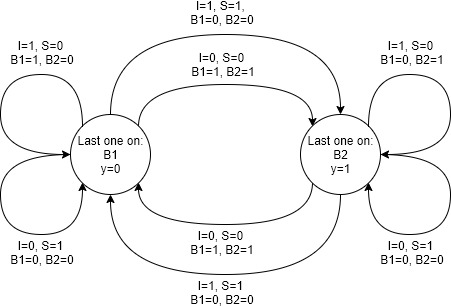
\includegraphics[width=0.7\textwidth]{../EJ1/Recursos/fsm_state_chart.jpg}
    \caption{Diagrama de estados para sistema de control de bombas.}
    \label{fig:fsm_state_chart_ex1}
\end{figure}

Como se puede observar, la máquina de estados planteada corresponde a una implementación de Mealy.
La decisión de utilizar esta implementación por sobre una de Moore, es que una aplicación estricta de la segunda, donde la salida dependiera únicamente del estado actual,
hubiera supuesto el uso de 6 estados, resultando altamente ineficiente en comparación a la solución elegida.\\
\\
La Tabla \ref{tab:truth_table_ex1} representa la tabla de verdad correspondiente a la máquina de estados en cuestión, donde \"y\" es el estado actual, \"I\" y \"S\" las entradas,
\"Y\" el siguiente estado a partir del próximo clock, y \"B1\" y \"B2\" las salidas asincrónicas. 
\begin{table}[H]
    \centering
    \begin{tabular}{ccc|ccc}
    \textbf{I} & \textbf{S} & \textbf{y} & Y & B1 & B2 \\ \hline
    0          & 0          & 0          & 1 & 1  & 1  \\
    0          & 0          & 1          & 0 & 1  & 1  \\
    0          & 1          & 0          & 0 & 0  & 0  \\
    0          & 1          & 1          & 1 & 0  & 0  \\
    1          & 0          & 0          & 0 & 1  & 0  \\
    1          & 0          & 1          & 1 & 0  & 1  \\
    1          & 1          & 0          & 1 & 0  & 0  \\
    1          & 1          & 1          & 0 & 0  & 0 
    \end{tabular}
    \caption{Tabla de verdad para máquina de estados de control de bombas.}
    \label{tab:truth_table_ex1}
    \end{table}

De la observación de las salidas, se infiere que los circuitos lógicos para implementarlas son los de las Figuras \ref{fig:Y_logic_circuit_ex5}, 
\ref{fig:B1_logic_circuit_ex5} y \ref{fig:B2_logic_circuit_ex5}.
Luego, la máquina de estados estará conformada por el circuito de la Figura \ref{fig:fsm_circtuit_ex5}.
\begin{figure}[H]
    \centering
    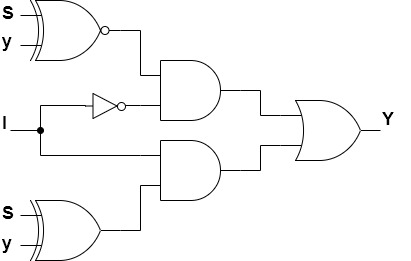
\includegraphics[width=0.6\textwidth]{../EJ1/Recursos/Y_logic_circuit.jpg}
    \caption{Circuito lógico para la entrada del Flip-Flop D.}
    \label{fig:Y_logic_circuit_ex5}
\end{figure}
\begin{figure}[H]
    \centering
    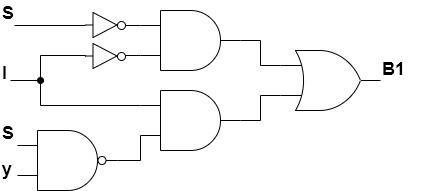
\includegraphics[width=0.6\textwidth]{../EJ1/Recursos/B1_logic_circuit.jpg}
    \caption{Circuito lógico para la salida de la bomba 1.}
    \label{fig:B1_logic_circuit_ex5}
\end{figure}
\begin{figure}[H]
    \centering
    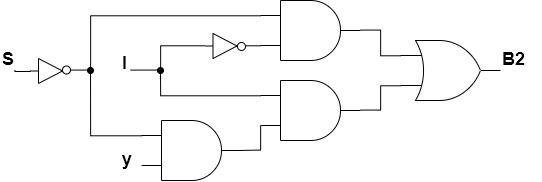
\includegraphics[width=0.6\textwidth]{../EJ1/Recursos/B2_logic_circuit.jpg}
    \caption{Circuito lógico para la salida de la bomba 2.}
    \label{fig:B2_logic_circuit_ex5}
\end{figure}
\begin{figure}[H]
    \centering
    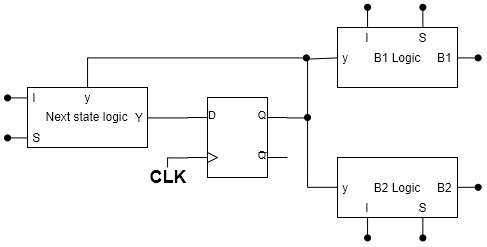
\includegraphics[width=0.7\textwidth]{../EJ1/Recursos/fsm_circuit.jpg}
    \caption{Circuito de la máquina de estados.}
    \label{fig:fsm_circtuit_ex5}
\end{figure}

	\newpage
	\section{Ejercicio 2: Reconocimiento de secuencia de bits}
	\newpage
	\section{Ejercicio 3: M\'aquina de Moore}
En esta secci\'on se desea dise\~ar una m\'aquina de estados implementada con m\'quina de Moore que cumpla con la mostrada en la Figura \ref{fig:TARGET}.
\begin{figure}[H]
    \centering
    \resizebox{0.8\textwidth}{!}{
    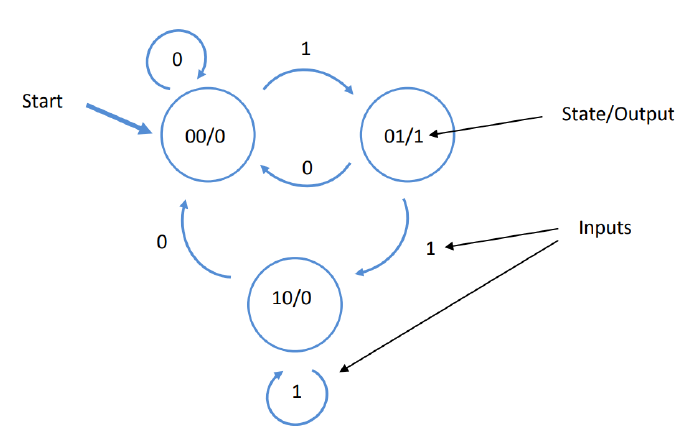
\includegraphics{../EJ3/Recursos/TARGET}
    }
    \caption{M\'aquina de estados en base a la cual se realiza el dise\~no}
    \label{fig:TARGET}
\end{figure}
Este comportamiento se corresponde con un detector de flancos que mantiene su salida en alto por un ciclo de \textit{clock}.
\subsection{Dise\~no de M\'aquina de Estados}
Se puede observar en la Tabla \ref{tab:STATE_TABLE} la tabla de estados correspondiente a la m\'aquina presentada en la Figura \ref{fig:TARGET}. Cabe aclarar que, en esta implementaci\'on se decide no fijar la salida en los estados no utilizados y utilizarlos como \textit{don't care} para facilitar el dise\~no.
\begin{table}[H]
    \centering
    \resizebox{0.4\textwidth}{!}{%
    \begin{tabular}{cccc}
    \hline
    Estado Actual & \multicolumn{2}{c}{Estado Siguiente} & Salida \\ \hline
    \multirow{2}{*}{$y_2$$y_1$} & $\omega=0$ & $\omega=1$ & \multirow{2}{*}{Z} \\
     & $Y_2$$Y_1$ & $Y_2$$Y_1$ &  \\ \hline
    00 & 00 & 01 & 0 \\
    01 & 00 & 10 & 1 \\
    10 & 00 & 10 & 0 \\
    11 & xx & xx & x \\ \hline
    \end{tabular}%
    }
    \caption{Tabla de estados de la máquina de Moore}
    \label{tab:STATE_TABLE}
\end{table}
Al haber 3 estados, es necesario utilizar 2 Flip Flops, en este caso D, para implementarla. 
Se resuelven entonces los mapas de Karnaugh para obtener el circuito que resuelve la Tabla \ref{tab:STATE_TABLE}.
\begin{figure}[H]
    \centering    
        \begin{Karnaughvuit}
        \maxterms{0,1,2,5,6}
        \minterms{4}
        \indeterminats{7, 3}
        \implicantsol{4}{red}
        \end{Karnaughvuit}
        \caption{Karnaugh para el estado siguiente $Y_1$}    
\end{figure}     
De este mapa se obtiene la soluci\'on que se muestra en \ref{eq:Y1}     
\begin{equation}
    Y_1 = \omega \cdot \overline{y_1}\cdot \overline{y_2}
    \label{eq:Y1}
\end{equation}      

\begin{figure}[H]
    \centering    
        \begin{Karnaughvuit}
        \maxterms{0,1,2,4}
        \minterms{5,6}
        \indeterminats{7, 3}

        \implicant{5}{7}{red}
        \implicant{7}{6}{blue}    

        \end{Karnaughvuit}
        \caption{Karnaugh para la variable $Y_2$}    
\end{figure}
De este mapa se obtiene la soluci\'on que se muestra en \ref{eq:Y2}  
\begin{equation}
    Y_2 = \omega \cdot y_1 + \omega \cdot y_2
    \label{eq:Y2}
\end{equation}
Adem\'as, es posible observar en la tabla de estados que $Z = y_1$. Si bien esto fija el valor de salida en el caso de que el estado actual fuera $y_2-y_1 = 1-1$, como en principio este estado no es v\'alido nunca deber\'ia suceder. Mas all\'a de esto, se define la salida como \textit{don't care} en ese caso, as\'i que tampoco presenta un problema.
Se presenta entonces, en la Figura \ref{fig:CIRCUIT}, el circuito l\'ogico obtenido a partir de resoluci\'on anterior.
\begin{figure}[H]
    \centering
    \resizebox{0.8\textwidth}{!}{
    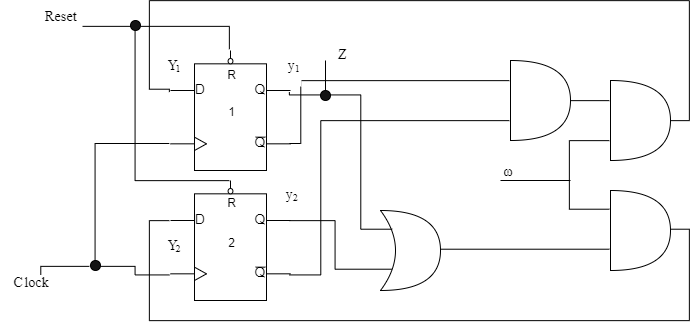
\includegraphics{../EJ3/Recursos/CIRCUIT}
    }
    \caption{Circuito implementado}
    \label{fig:LEVEL_SHIFTER}
\end{figure}
Se puede observar que se agrega una entrada adicional de reset, para poder resetear los flipflops al iniciar, comenzando en un estado v\'alido

\subsection{Level Shifters}
Si bien entradas y salidas del circuito son de 5V-0V, se dise\~na la l\'ogica interna de la m\'aquina de estados para que funcione a 3.3V. Se utilizan con este fin \textit{level shifters} en  las entradas y salidas del sistema.
Luego de contrastar el funcionamiento de las opciones disponibles que cumplen con lo requerido, se concluye que la de mejor funcionamiento en cuanto a sus caracter\'isticas, como tiempo de propagaci\'on y tiempo de rise, es presentada en la Figura \ref{fig:LEVEL_SHIFTER}.

\begin{figure}[H]
    \centering
    \resizebox{0.8\textwidth}{!}{
    \includegraphics{../EJ3/Recursos/mos_interface}
    }
    \caption{Level shifter utilizado}
    \label{fig:LEVEL_SHIFTER}
\end{figure}
\subsection{Regulador de tensi\'on}
Para obtener una tensi\'on constante en 3.3V, que se utilizan tanto  para la alimentaci\'on de los circuitos integrados, como para los \textit{level shifters}, se implementa un regulador de tensi\'on simple con un diodo zener y una resistencia.
A pesar de que el regulador funciona correctamente, se observa como un fallo en su dise\~no que la corriente que consume es muy elevada. Se asume este defecto a la baja resistencia utilizada en el regulador. 
\subsection{Mediciones y resultados}
Se puede ver en la Figura \ref{fig:GRAPH1} se puede ver como responde la m\'aquina de estados ante una entrada que se mantiene en alto por menos de un ciclo de clock, es decir, del estado 0-0 al estado 0-1 y de nuevo al estado 0-0.

\begin{figure}[H]
    \centering
    \resizebox{0.8\textwidth}{!}{
    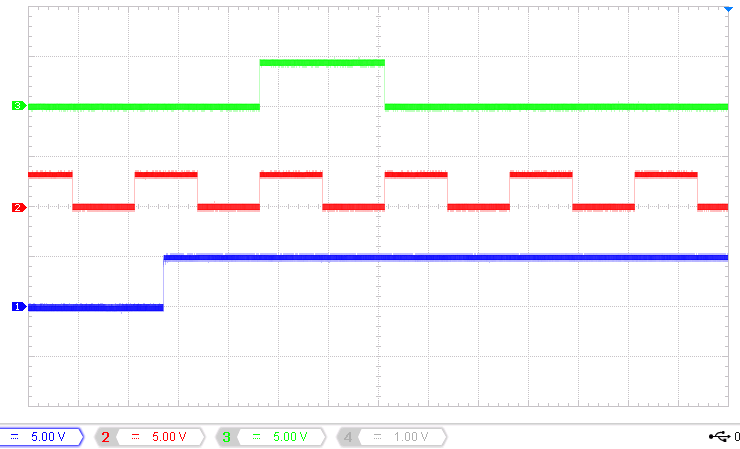
\includegraphics{../EJ3/Recursos/FOTO1}
    }
    \caption{del estado 0-0 al estado 0-1 y de nuevo al estado 0-0..Entrada en azul, clock en rojo y salida en verde}
    \label{fig:GRAPH1}
\end{figure}

En la Figura \ref{fig:GRAPH2} se observa la respuesta de la m\'aquina de estados a una entrada que se mantiene en alto por m\'as tiempo del que dura un per\'iodo del clock, es decir la transici\'on 0-0, 0-1, 1-0.
\begin{figure}[H]
    \centering
    \resizebox{0.8\textwidth}{!}{
    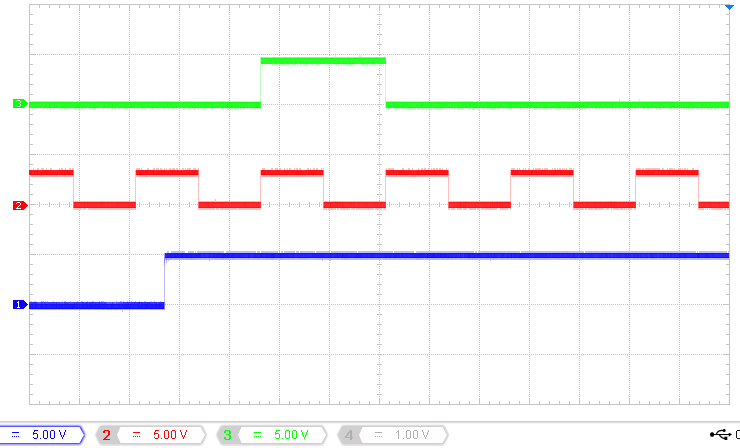
\includegraphics{../EJ3/Recursos/FOTO2}
    }
    \caption{Transici\'on 0-0, 0-1, 1-0. Entrada en azul, clock en rojo y salida en verde}
    \label{fig:GRAPH2}
\end{figure}

Se puede observar que en todos los casos el sistema responde en concordancia con lo esperado.
\end{document}
